\documentclass[compress]{beamer}
\usepackage[utf8]{inputenc}
\usepackage[francais]{babel}
\usepackage[T1]{fontenc}
\usepackage{amssymb}
\usepackage{amsmath}
\usepackage{amsfonts}
\usepackage{hyperref}
\usepackage[]{algorithm2e}
\usepackage{amssymb}
\usepackage{verbatim}
\usepackage{listings}
\usepackage{color}
\usepackage{graphicx}
\usetheme[navigation]{UMONS}

\author{Clément Tamines, Florent Delgrange}
\title{Temps, Horloge et l'ordonnancement de évènements dans un système distribué}

\setbeamercovered{transparent} 
\setbeamertemplate{navigation symbols}{} 
\institute{UMONS\\Faculté des Sciences\\MA1 Sciences Informatiques\\[2ex]
  
\includegraphics[height=4ex]{UMONS}\hspace{2em}%
  \raisebox{-1ex}{
\includegraphics[height=6ex]{UMONS_FS}}}
\date{novembre 2016} 
\definecolor{darkgreen}{rgb}{0.0, 0.2, 0.13}
\subject{Réseaux II} 

\begin{document}

\begin{frame}
\titlepage
\end{frame}

\begin{frame}
\tableofcontents
\end{frame}

\section{Introduction}

\begin{frame}
\begin{itemize}
\item Comment classer chronologiquement les évènements dans un système distribué ?
\item Comment définir le fait qu'un évènement A s'est passé avant un autre évènement B ?
\end{itemize}
\end{frame}

\begin{frame}
\frametitle{Système distribué}
	\begin{definition}
		Un système distribué est une collection de processus distincts qui sont séparés dans l'espace et qui communiquent entre eux par 			messages.
	\end{definition}
	Exemples : 
	\begin{itemize}
		\item Système de PC inter-connectés à l'aide d'un réseau de communication
		\item Un simple PC dans lequel l'unité de contrôle , les unités de mémoire et les canaux d'entrées/sorties sont des processus séparés.
		\item etc
	\end{itemize}
\end{frame}

\begin{frame}
\frametitle{Temps et ordonnancement ?}
Soient a et b, deux évènements. On dit que\\
\textit{a est arrivé avant b} si $a$ est arrivé plus tôt dans le temps que $b$.\\
\textbf{Horloge réelle : }n'est pas forcément exacte et ne fournit pas le temps au sens physique précis ! $\implies$ la relation \textit{est arrivé avant} doit s'exprimer sans horloge réelle.\\
$\implies$ la relation \textit{est arrivé avant} doit s'exprimer sans horloge réelle.
\end{frame}

\section{Ordre partiel}

\begin{frame}
\frametitle{\'Evènements}
Le système est composé d'une collection de processus et chaque processus est une séquence d'évènements.\\
exemple : L'exécution d'un sous-programme ou d'une instruction sur un ordinateur peut être considéré comme un évènement.\\
Les évènements d'un processus forment une séquence où a apparait avant b ssi a est exécuté avant b.
\begin{figure}
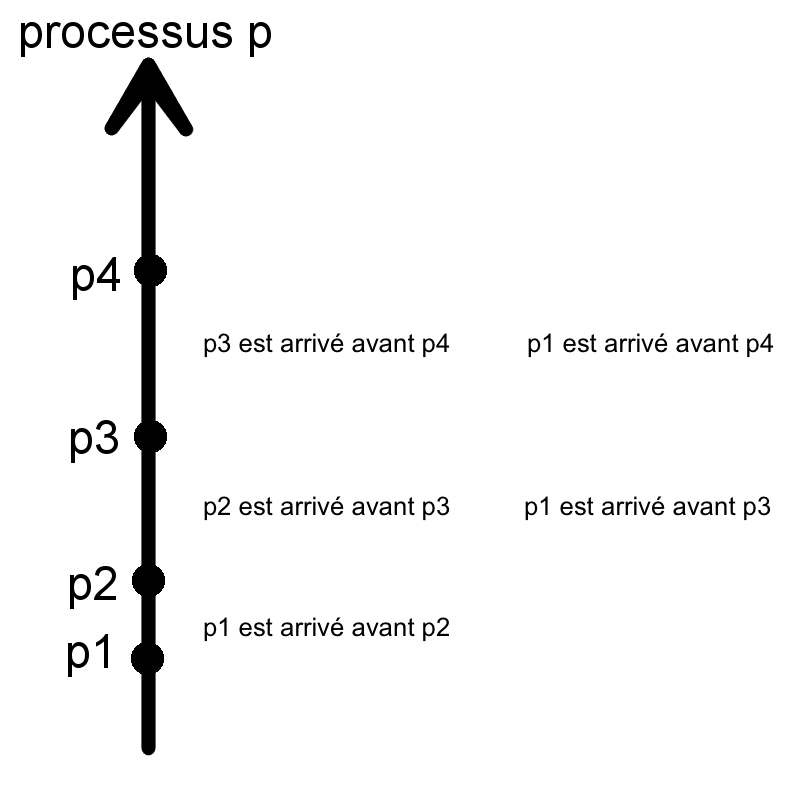
\includegraphics[scale=0.15]{process1.png}
\end{figure}

\end{frame}
\end{document}